% Copyright 2016 - 2019 Bas van Meerten and Wouter Franssen
%
%This file is part of ssNake.
%
%ssNake is free software: you can redistribute it and/or modify
%it under the terms of the GNU General Public License as published by
%the Free Software Foundation, either version 3 of the License, or
%(at your option) any later version.
%
%ssNake is distributed in the hope that it will be useful,
%but WITHOUT ANY WARRANTY; without even the implied warranty of
%MERCHANTABILITY or FITNESS FOR A PARTICULAR PURPOSE.  See the
%GNU General Public License for more details.
%
%You should have received a copy of the GNU General Public License
%along with ssNake. If not, see <http://www.gnu.org/licenses/>.

\documentclass[11pt,a4paper]{article}
% Copyright 2016 - 2017 Bas van Meerten and Wouter Franssen
%
%This file is part of ssNake.
%
%ssNake is free software: you can redistribute it and/or modify
%it under the terms of the GNU General Public License as published by
%the Free Software Foundation, either version 3 of the License, or
%(at your option) any later version.
%
%ssNake is distributed in the hope that it will be useful,
%but WITHOUT ANY WARRANTY; without even the implied warranty of
%MERCHANTABILITY or FITNESS FOR A PARTICULAR PURPOSE.  See the
%GNU General Public License for more details.
%
%You should have received a copy of the GNU General Public License
%along with ssNake. If not, see <http://www.gnu.org/licenses/>.

\usepackage[british]{babel}
\usepackage{graphicx,booktabs,listings,amsmath,pgfplots,pgfplotstable}
\usepackage[small,bf,nooneline]{caption}
\usepackage{subcaption}
\usepackage[sort&compress,numbers]{natbib}
\usepackage{tikz}
\usepackage{mathtools}
\usepackage[nottoc]{tocbibind}%adds bibliography to table of contents.
\graphicspath{{./images/}}
%\setlength{\textwidth}{453pt} %597 pt is the a4 paperwidth. Minus 2 in margin. 72 pt = 1 in
%\setlength{\hoffset}{-\oddsidemargin}
%\setlength{\voffset}{-30pt} %
%\setlength{\textheight}{651 pt} %a4 height 845 pt minus 2* total headheight. In this case 2*88pt
%% examine margines via the layout package. Use command \layout{} in document to draw a picture.
%\setlength{\parindent}{0.5 cm}
%\setlength{\parskip}{0 cm}
\usepackage[left=82pt,right=82pt,top=95pt,bottom=95pt,footnotesep=0.5cm]{geometry}
%\setlength{\headheight}{14pt}

%define colours--------------------
%dark
\usepackage{xcolor}
\definecolor{MyGrayD}{RGB}{1,1,1}
\definecolor{MyRedD}{RGB}{237,45,46}
\definecolor{MyGreenD}{RGB}{0,140,71}
\definecolor{MyBlueD}{RGB}{24,89,169}
\definecolor{MyOrangeD}{RGB}{243,125,34}
\definecolor{MyPurpleD}{RGB}{102,44,145}
\definecolor{MyBrownD}{RGB}{161,29,32}
\definecolor{MyPinkD}{RGB}{179,56,147}
%normal
\definecolor{MyGray}{RGB}{114,114,114}
\definecolor{MyRed}{RGB}{241,89,95}
\definecolor{MyGreen}{RGB}{121,195,106}
\definecolor{MyBlue}{RGB}{89,154,211}
\definecolor{MyOrange}{RGB}{249,166,90}
\definecolor{MyPurple}{RGB}{158,102,171}
\definecolor{MyBrown}{RGB}{205,112,88}
\definecolor{MyPink}{RGB}{215,127,179}
%light
\definecolor{MyGrayL}{RGB}{204,204,204}
\definecolor{MyRedL}{RGB}{242,174,172}
\definecolor{MyGreenL}{RGB}{216,228,170}
\definecolor{MyBlueL}{RGB}{184,210,235}
\definecolor{MyOrangeL}{RGB}{242,209,176}
\definecolor{MyPurpleL}{RGB}{212,178,211}
\definecolor{MyBrownL}{RGB}{221,184,169}
\definecolor{MyPinkL}{RGB}{235,191,217}
%----------------------------------

%Figure ref with hyperref
\newcommand{\fref}[1]{\hyperref[#1]{Figure \ref*{#1}}}
\newcommand{\sref}[1]{\hyperref[#1]{Section \ref*{#1}}}
\newcommand{\tref}[1]{\hyperref[#1]{Table \ref*{#1}}}

%Makes a new command for figures with input values: filename, width(times linewidth),
% caption and label.
\newcommand{\onefigure}[4]{
\setlength{\captionwidth}{#2\linewidth}
\begin{figure}
\includegraphics[width=#2\linewidth]{#1}
\centering
\parbox{\linewidth}{\caption{#3}
\label{#4}}
\end{figure}
}

%Makes a new command for tikz figures with input values: tikz commands, 
% caption and label.
\newcommand{\onetikz}[3]{
\settowidth{\captionwidth}{#1}
\ifthenelse{\lengthtest{\captionwidth<0.7\linewidth}}{\setlength{\captionwidth}{0.7\linewidth}}{}

\begin{figure}
\centering
#1
\centering
\parbox{\linewidth}{\caption{#2}
\label{#3}}
\end{figure}
}

%Makes a new command for two figures next to each other with input values: filename1, caption1, label1,filename2, caption2 and label2. Figure width is set to 0.47\linewidth and the space between the figures is filled with \hfill so the sides of the figures align with to edge of the line.
\newcommand{\twofigure}[6]{
\setlength{\captionwidth}{\linewidth}
\begin{figure*}[ht!]
\begin{minipage}[t]{0.47\linewidth}
\includegraphics[width=\linewidth]{#1}
\centering
\caption{#2}
\label{#3}
\end{minipage}
\hfill
\begin{minipage}[t]{0.47\linewidth}
\centering
\includegraphics[width= \linewidth]{#4}
\centering
\caption{#5}
\label{#6}
\end{minipage}
\end{figure*}
}


%Makes a new command for a table with caption witdh equal to the total table width. Input: tabular, caption and label. Example:
%\onetable{
%\begin{tabular}{ccc}
%a&b&c\\
%\hline
%1&1&1\\
%1&1&1\\
%1&1&1\\
%\end{tabular}
%{The caption.}
%{tab:table1}
%}
\newcommand{\onetable}[3]{
\settowidth{\captionwidth}{#1}
\ifthenelse{\lengthtest{\captionwidth<0.7\linewidth}}{\setlength{\captionwidth}{0.7\linewidth}}{}
\begin{table}
\caption{#2}
\vspace{-0.24cm} %Puts caption close to toprule
\label{#3}
\centering
#1
\end{table}
}

%Makes a long table with captionwidth equal to tablewidth. It takes the following arguments:
%1: Column specifier (e.g. cccc)
%2: Caption
%3: Label
%4: First head (i.e. first row of regular table)
%5: Head of consecutive pages
%6: Foot of pagebreak
%7: Lastfoot (e.g. \midrule)
%8: Body of table
\newcommand{\onelongtable}[8]{
\begin{center}
\settowidth{\captionwidth}{
\begin{tabular}{#1}
#4
#8
\end{tabular}} % This ends the captionwidth part. Next comes the real table.

\begin{longtable}{#1}
\caption{#2}\\
\vspace{-0.74cm} %Puts caption close to toprule
\label{#3}\\

#4
\endfirsthead

#5
\endhead

#6
\endfoot

#7
\endlastfoot

#8
\end{longtable}
\end{center}}




%1:pgfplots code
%2:width
%3:caption
%4:label
\newcommand{\pgfplotsfigure}[4]{
\pgfplotsset{width=#2\linewidth}
\setlength{\captionwidth}{#2\linewidth}
\begin{figure}[t]
\centering
#1
\centering
\parbox{\linewidth}{\caption{#3}
\label{#4}}
\end{figure}
}


\usepackage[bitstream-charter]{mathdesign}
\usepackage[T1]{fontenc}
\usepackage[protrusion=true,expansion,tracking=true]{microtype}
\pgfplotsset{compat=1.7,/pgf/number format/1000 sep={}, axis lines*=left,axis line style={gray},every outer x axis line/.append style={-stealth'},every outer y axis line/.append style={-stealth'},tick label style={font=\small},label style={font=\small},legend style={font=\footnotesize}}
\usepackage{colortbl}
\usetikzlibrary{calc}

%Set section font
\usepackage{sectsty}
\allsectionsfont{\color{black!70}\fontfamily{SourceSansPro-LF}\selectfont}
%--------------------


%Set toc fonts
\usepackage{tocloft}
%\renewcommand\cftchapfont{\fontfamily{SourceSansPro-LF}\bfseries}
\renewcommand\cfttoctitlefont{\color{black!70}\Huge\fontfamily{SourceSansPro-LF}\bfseries}
\renewcommand\cftsecfont{\fontfamily{SourceSansPro-LF}\selectfont}
%\renewcommand\cftchappagefont{\fontfamily{SourceSansPro-LF}\bfseries}
\renewcommand\cftsecpagefont{\fontfamily{SourceSansPro-LF}\selectfont}
\renewcommand\cftsubsecfont{\fontfamily{SourceSansPro-LF}\selectfont}
\renewcommand\cftsubsecpagefont{\fontfamily{SourceSansPro-LF}\selectfont}
%--------------------


\usepackage[hidelinks,colorlinks,allcolors=black, pdftitle={Fitting Czjzek distribution spectra in ssNake},pdfauthor={Wouter M.J.\ Franssen}]{hyperref}

\interfootnotelinepenalty=10000 %prevents splitting of footnote over multiple pages
\linespread{1.2}

\title{\color{black}\fontfamily{SourceSansPro-LF}\bfseries Fitting Czjzek spectra distribution in ssNake}
\author{}
\date{\color{black}\fontfamily{SourceSansPro-LF}\bfseries \today}


\begin{document}
%\newgeometry{left=72pt,right=72pt,top=95pt,bottom=95pt,footnotesep=0.5cm}
\microtypesetup{protrusion=true} % enables protrusion

\maketitle

\section{Introduction}
This tutorial describes how to fit Czjzek and Extended Czjzek quadrupolar lineshapes in ssNake. As this is relatively advanced, it is recommended to study the tutorial on CSA fitting and the single fit part of MultiFitQuadrupole first.

A Czjzek lineshape occurs in case where this is a atomic site in a material with considerable distortions around it. This standard Czjzek model assumes a site with in first instance no quadrupolar coupling ($C_\text{q}=0$) due to symmetry. However, the distortions in the material break the symmery and introduce a quadrupolar coupling.

Simulating a Czjzek lineshape is more involved, as it requires calculation of a whole series of quadrupolar powder patterns (the distortion is different for different positions in the material). Based on the parameters of the Czjzek distribution, the relative intensity of each of these powder patterns changes. To be able to calculate this efficiently in an iterative routine, ssNake pre-calculates the quadrupole powder patterns. In the fitting, the Czjzek parameters change, but this leads only to a different sum of the powder patterns. The collection of pre-calculated lineshapes is called the `library'.

Generating this library can be done by ssNake itself, or supplied by the user from an external source. (In the ssNake paper, we used SIMPSON to calculate lineshape with excitation efficiencies include, for example.) It is in the generation of the library that settings regarding Magic Angle Spinning, inclusion of satellite intensities etc.\ are relevant.

When generating the library, a grid with quadrupolar settings must be chosen: for $C_\text{q}$ and $\eta$. The smaller the steps that are taken, the more accurate the fitting, at the expense of speed. Note that while $\eta$ is of course always between 0 and 1, $C_\text{q}$ can take any positive value. Generally, Czjzek lineshapes are accurately calculated for $C_\text{q}^\text{max} = 4\sigma$, with $\sigma$ the Czjzek width. As $\sigma$ can change during the fitting, the choice for $C_\text{q}^\text{max}$ should be revisited after the fitting. If this value is unsuitable for the fit results, a new library must be generated and the fitting rerun.

Additional issues can arise if multiple Czjzek sites are simulated. In this case, the total width of the 
$C_\text{q}$ range must be wide enough to accommodate the larger of the two $\sigma$ values, while the step size must be small enough to accurately describe the distribution due to the small $\sigma$.

In the following tutorial, we will generate the library and fit an experimental data set with both a regular Czjzek, as well as an Extended Czjzek distribution.


\section{Data}
The data used in this tutorial is a $^{35}$Cl spectrum of ball-milled MgCl$_2$ with a diisobutyl phthalate adduct. The spectrum was acquired on a 20 T magnet at a spinning speed of 15.625 kHz.


\section{Fitting a Czjzek lineshape}
Start by loading the data supplied with this tutorial: `MgCl2.mat'. We observe a central transition with some spinning sidebands. The shape of the central transition is not really clear, indicating it is not just a single quadrupolar site. Fitting it in this way therefore does not lead to a good result:

\begin{center}
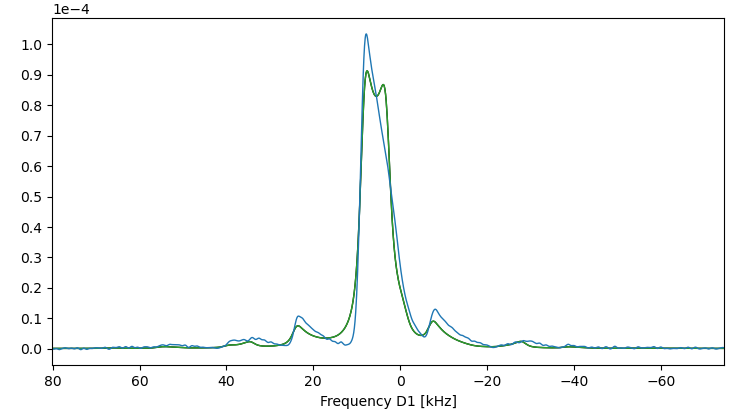
\includegraphics[width=0.8\linewidth]{Figs/fig1.PNG}
\end{center}

We therefore need something more complicated: the Czjzek routine!.
\begin{itemize}
  \item Set the x-axis to ppm using the bottom frame. 
  \item Open the Czjzek fitting routine using `Fitting $\longrightarrow$ Czjzek'.
\end{itemize}

Firstly, we must generate a library, as was explained above.

\begin{itemize}
  \item Click the 'Library' button.
\end{itemize}
This show the following:
\begin{center}
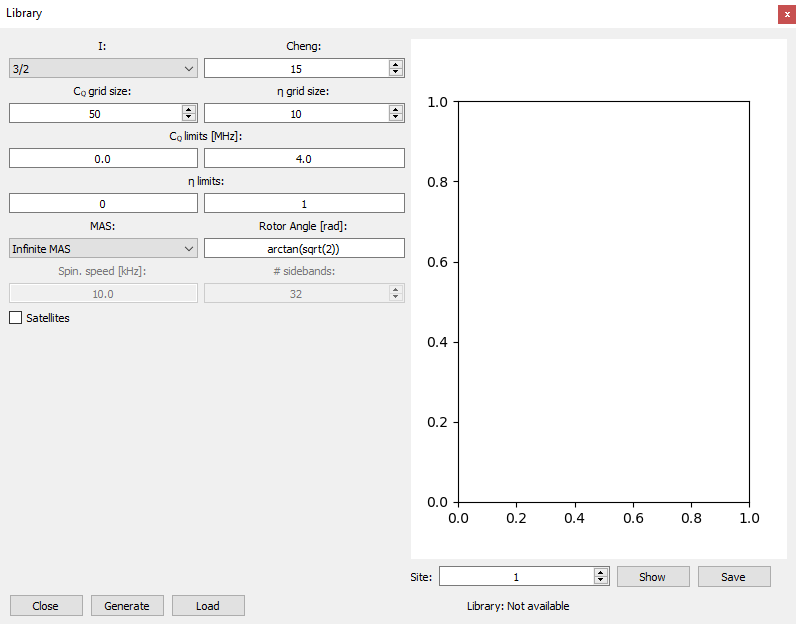
\includegraphics[width=0.8\linewidth]{Figs/fig2.PNG}
\end{center}
Here, we can fill in the settings for our library, and generate it. The plot on the right can be used to view the Czjzek amplitude on the chosen $C_\text{Q}$-$\eta$ grid. For this, it use the largest $\sigma$-value that was put in the fitting window. This value is till at its default, so we have no clue about the grid size\ldots

Push the `Show' button on the right gives the Czjzek intensities for the current $\sigma$ value:
\begin{center}
\includegraphics[width=0.5\linewidth]{Figs/fig3.PNG}
\end{center}

The distribution is nicely centered on the x-axis, so for the current $\sigma$ this is a good grid.

Now, to generate the library, we need a couple of experimental settings:
\begin{itemize}
  \item Set `MAS' to `Finite MAS'.
  \item Set the `Spin. Speed' to 15.625 kHz.
  \item Set the `\# sidebands' to 16.
\end{itemize}
These are all the changes we need for now. Generate the library by pushing `Generate'. This can take some time. After this, close the window.

Pushing `Sim' in the fitting window gives us the current simulated spectrum:
\begin{center}
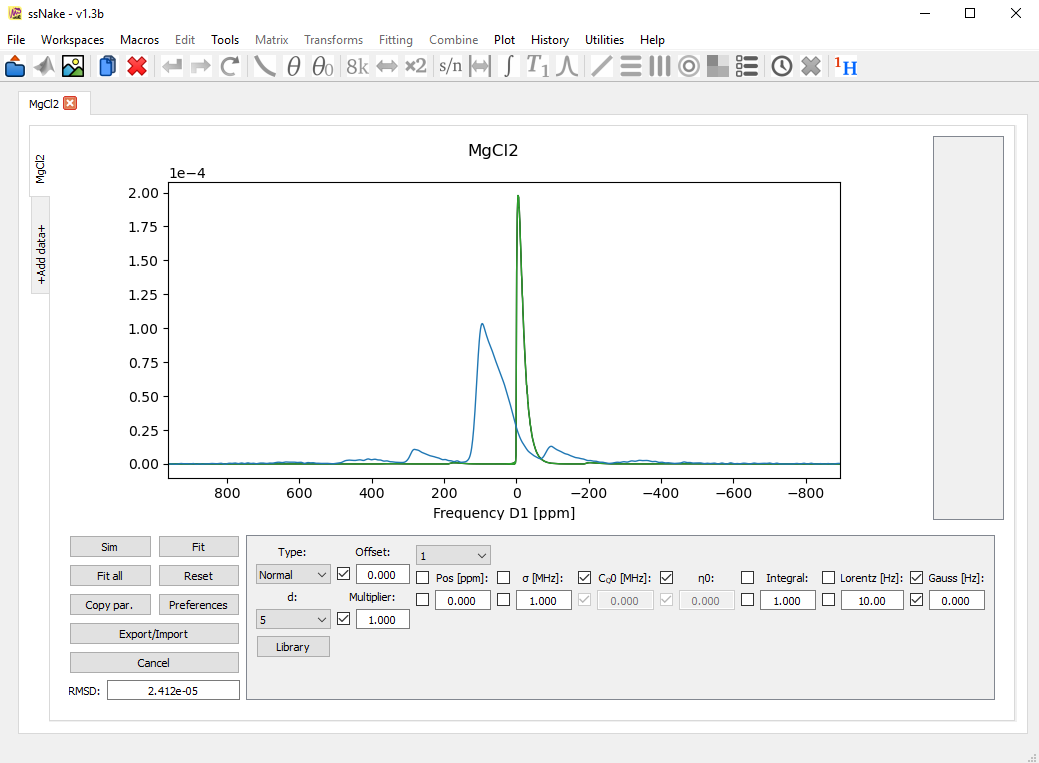
\includegraphics[width=0.8\linewidth]{Figs/fig4.PNG}
\end{center}

The quadrupolar coupling in the experimental spectrum is a bit more than in the simulation, so we need to change that a bit. Also, the position is off:
\begin{itemize}
  \item Set `$\sigma$' to 2 MHz.
  \item Set `Pos' to 100 ppm.
  \item Push `Sim'.
\end{itemize}
This gives:
\begin{center}
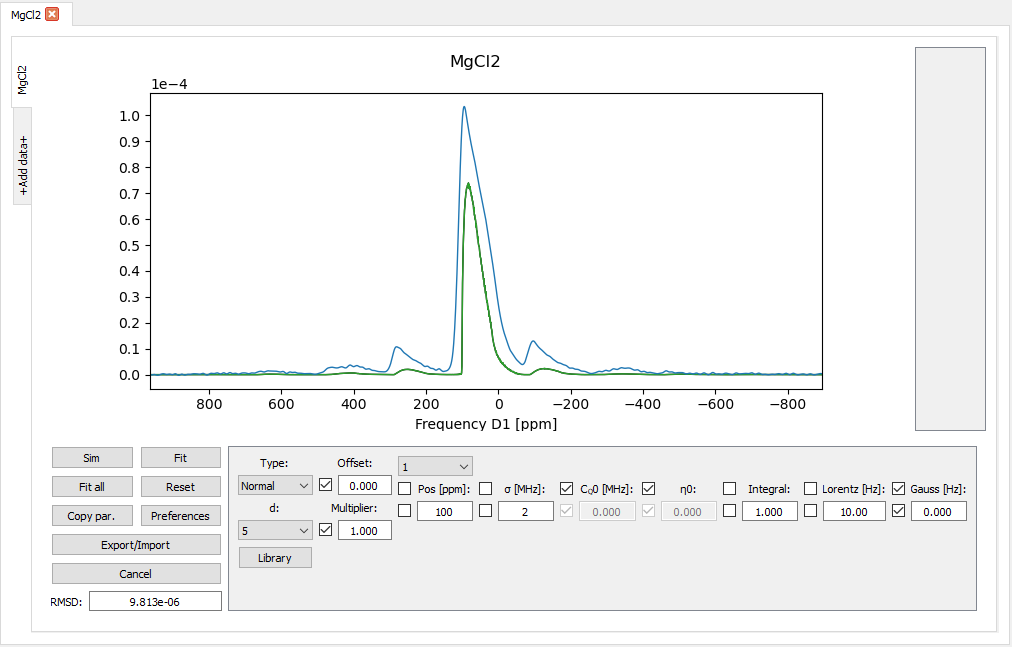
\includegraphics[width=0.8\linewidth]{Figs/fig5.PNG}
\end{center}
This looks ok. In must fitting routines, we would now push `Fit' and be done. However, as we have double $\sigma$ the library might be wrong! We need twice the $C_\text{Q}$ range now.

Open the Library window again, and push `Show' on the right. This shows:
\begin{center}
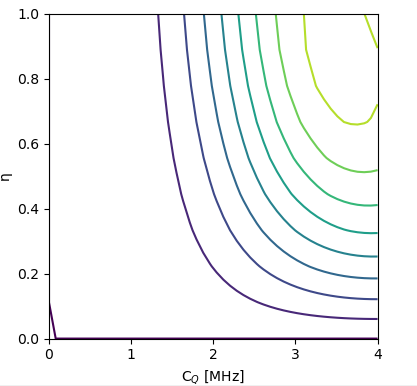
\includegraphics[width=0.5\linewidth]{Figs/fig6.PNG}
\end{center}
Not good! To fix this, we need a wider range:
\begin{itemize}
  \item Set the $C_\text{Q}$ limit maximum to 10 MHz.
\end{itemize}
This leads to (after `Show'):

\begin{center}
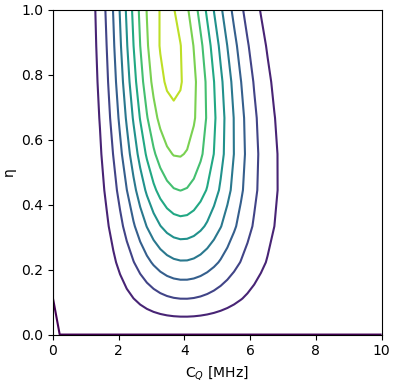
\includegraphics[width=0.5\linewidth]{Figs/fig7.PNG}
\end{center}
Much better! I put the range a bit more than just times 2, to be able to accommodate a large $\sigma$ if this happens during the fit.
\begin{itemize}
  \item Push `Generate' to generate the new library.
  \item Close the window.
\end{itemize}
Now, let's fit:
\begin{itemize}
  \item Untick the Gauss value, and set it to 1000 Hz.
  \item Set `Integral' to 2.
  \item Push `Fit'.
\end{itemize}

This gives:
\begin{center}
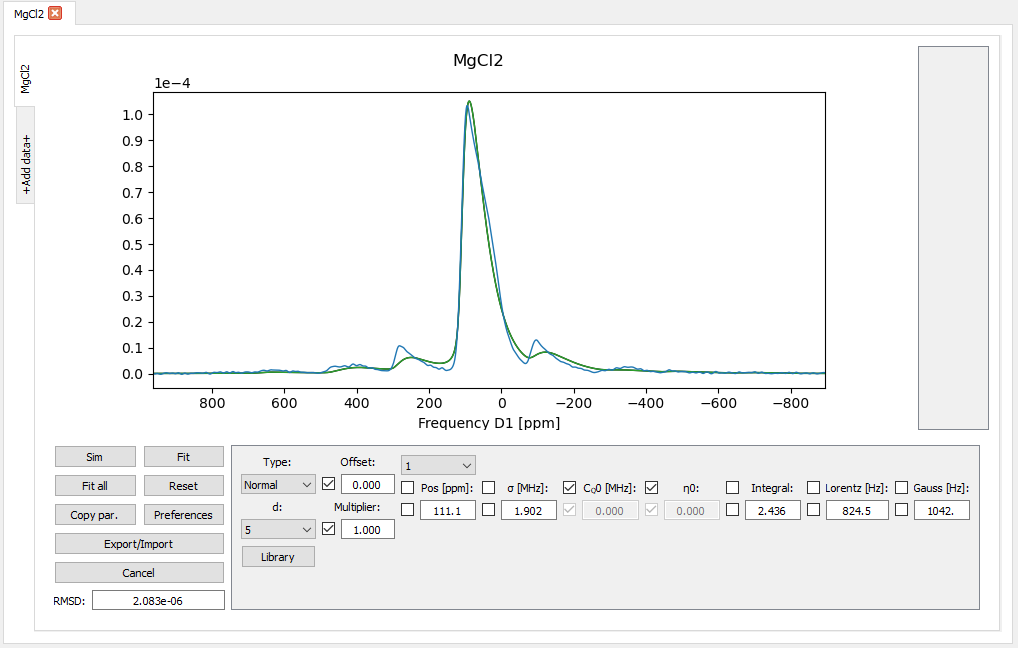
\includegraphics[width=0.8\linewidth]{Figs/fig8.PNG}
\end{center}
Which is much better than the regular quadrupolar fit shown above. However, the result is not that great. The sidebands for example are much `sharper' in the experimental spectrum\ldots The reason why this is, is because the underlying quadrupolar pattern has a $C_\text{Q}$ value of its own.
\begin{itemize}
  \item Change the `Type' to Extended.
\end{itemize}
This actives two new parameters. $C_\text{Q}^0$ and $\eta^0$. Put these at 4 MHz and 0, respectively. (These parameters relate to the undisturbed value of the material. As the data was recorded on a compound based on MgCl$_2$, the values of pure MgCl$_2$ are a good place to start. Based on this structure we also choose $\eta^0=0$.) Also, untick the box at $C_\text{Q}^0$ to let the fitting optimize it.
\begin{itemize}
  \item Set Lorentz back to 100, and Gauss back to 1000.
  \item Push `Sim'. This will take some time.
\end{itemize}
Noticed how long that took? This is because the calculation of the Extended Czjzek distribution is very involved (it requires integration over three angles). We have $\eta^0=0$, which means ssNake is actually using its fast routine! It can be even slower.

The spectrum we get looks like:
\begin{center}
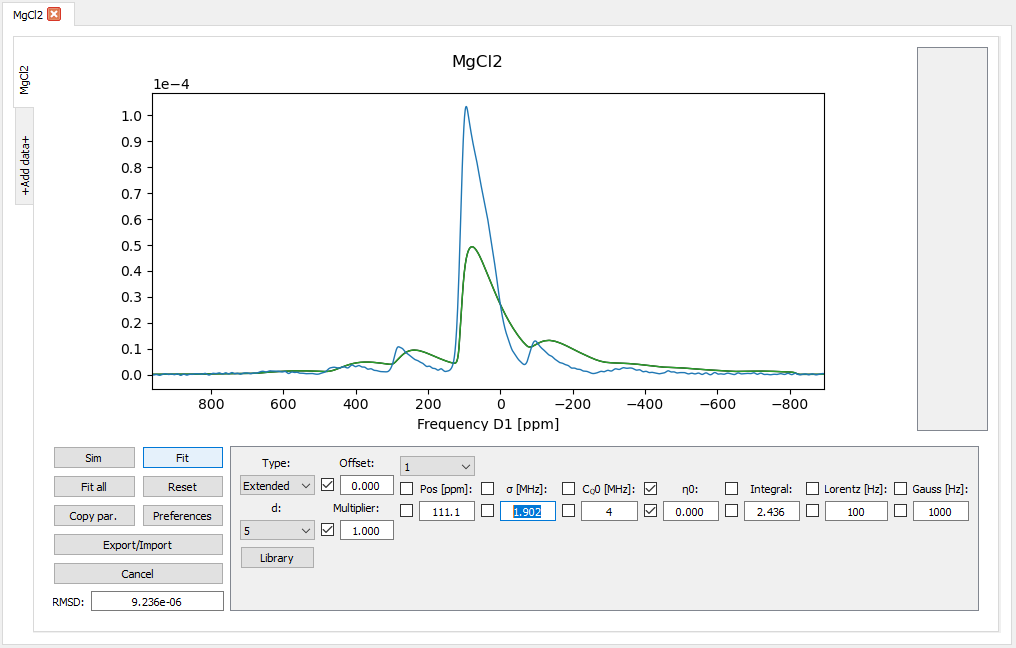
\includegraphics[width=0.8\linewidth]{Figs/fig9.PNG}
\end{center}
The center line looks a bit too broad and smeared out. Perhaps $\sigma$ is now too high?
\begin{itemize}
  \item Set $\sigma$ to 0.8 MHz.
  \item Push `Sim'.
\end{itemize}
Much better:
\begin{center}
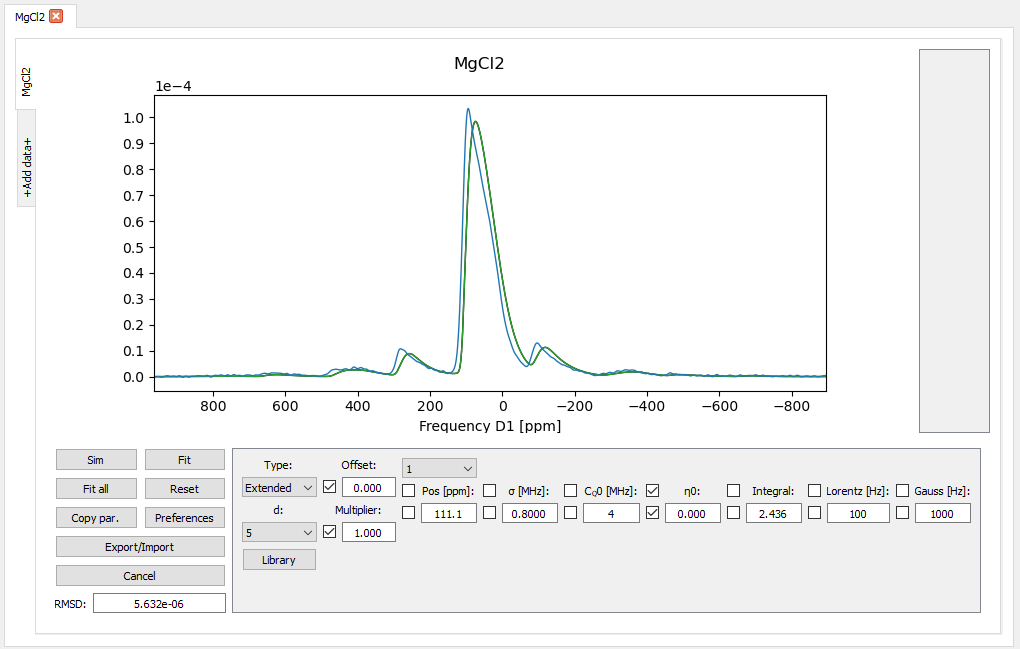
\includegraphics[width=0.8\linewidth]{Figs/fig10.PNG}
\end{center}
A quick check of the Library shows that we are still in a good regime for the simulation.
\begin{center}
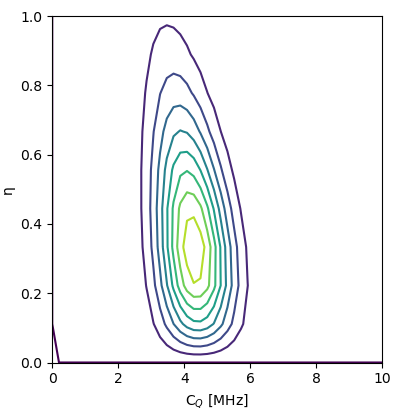
\includegraphics[width=0.5\linewidth]{Figs/fig11.PNG}
\end{center}
(Notice the different shape of the contours: this is due to the Extended changes.)

This means that we can fit!
\begin{itemize}
  \item Push `Fit'.
  \item Grab a cup of coffee: this will take some time. The underlying routine is multithreaded, meaning that all your CPU cores will be used. If you have the `numba' python library installed, the calculations will be a lot faster. (This is bundled in the ssNake installer.)
\end{itemize}
After some time we get:
\begin{center}
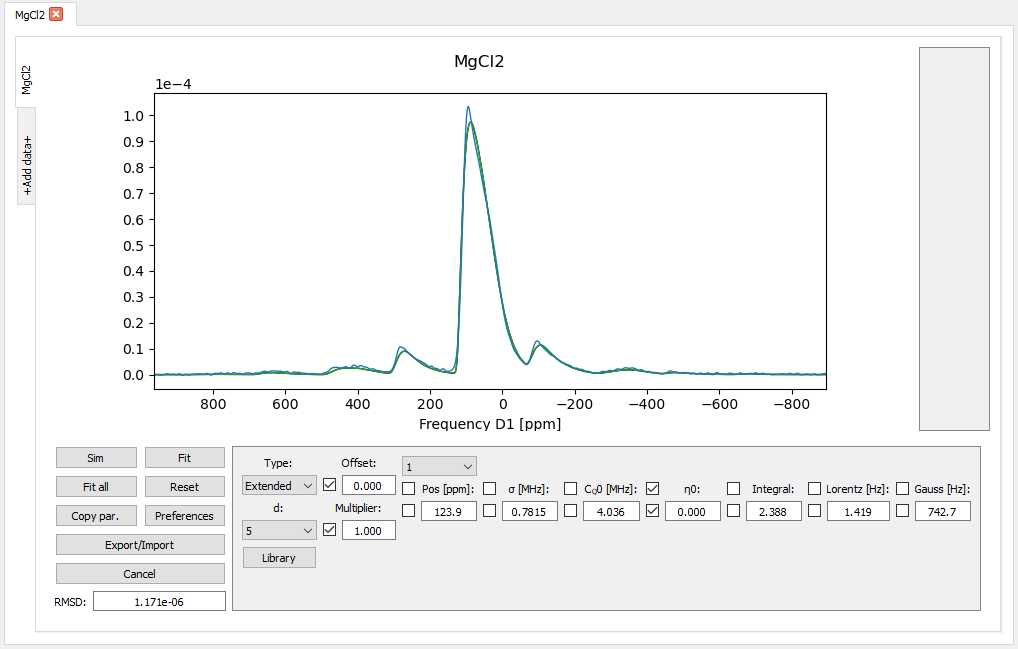
\includegraphics[width=0.8\linewidth]{Figs/fig12.PNG}
\end{center}
which is a quite good fit. Definitely much better than the quadrupolar or normal Czjzek fit. The fit result can also be found in the data directory of this tutorial.

As a nice trick, we can also disable the extended Czjzek addition, and simulate again. This leads to (after lowring the integral a bit):
\begin{center}
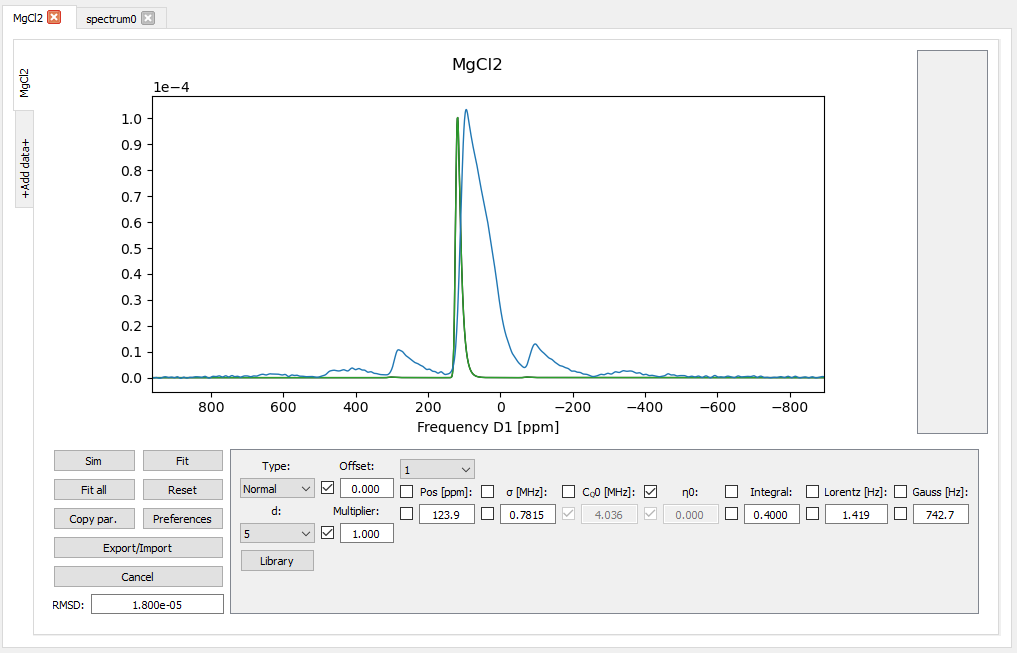
\includegraphics[width=0.8\linewidth]{Figs/fig13.PNG}
\end{center}
Clearly, the width of the line is mostly due to the standard quadrupolar broadening. The Czjzek effect is much smaller than we initially had ($\sigma=2$ MHz). The same broadening of the line can however not be caused by Lorentzian or Gaussian broadening. It really is a distribution in quadrupolar parameters.

This concludes this tutorial. The take home message is that regular Czjzek fitting can be done in a short time, due to the use of a library. Extended Czjzek fitting requires some patience. In both cases, it is important to check, after a change in the parameters, whether the library we use is still correct.


\end{document}
